
\documentclass[12pt]{book}
\usepackage[a4paper,top=3cm,bottom=3cm]{geometry}
\usepackage{graphicx} 

\makeatletter
\newcommand{\judul}[1]{%
  {\parindent \z@ \centering \normalfont
    \interlinepenalty\@M \Large \bfseries #1\par\nobreak \vskip 20\p@ }}
\newcommand{\subjudul}[1]{%
  {\parindent \z@ \normalfont
    \interlinepenalty\@M \bfseries #1\par\nobreak \vskip 20\p@ }}
\newcommand{\lagu}[1]{%
  {\parindent \z@ \normalfont
    \interlinepenalty\@M \bfseries \emph{#1}\par\nobreak \vskip 20\p@ }}

\renewenvironment{description}
               {\list{}{\labelwidth\z@ \itemindent-\leftmargin
                        \let\makelabel\descriptionlabel}}
               {\endlist}
\renewcommand*\descriptionlabel[1]{\hspace\labelsep 
                                \normalfont\bfseries #1 }
    

\makeatother

\newcommand{\BU}[1]{\begin{itemize} \item[U:] #1 \end{itemize}}
\newcommand{\BI}[1]{\begin{itemize} \item[I:] #1 \end{itemize}}
\newcommand{\BP}[1]{\begin{itemize} \item[P:] #1 \end{itemize}}
% \newcommand{\BL}[1]{\begin{itemize} \item[Wawan:] #1 \end{itemize}}
% \newcommand{\BW}[1]{\begin{itemize} \item[Novi:] #1 \end{itemize}}
% \newcommand{\BMP}[1]{\begin{itemize} \item[W+N:] #1 \end{itemize}}
% \newcommand{\BS}[1]{\begin{itemize} \item[Saksi:] #1 \end{itemize}}
\newcommand{\keluargatri}{Fransiskus de Sales Noer Susilo }
\newcommand{\keluargatra}{Andreas Puji Hesti Sasmito }
\newcommand{\romo}{H. Asodo, OMI }
\newcommand{\camantri}{Ignatia Dinar Melani }
\newcommand{\camantra}{Ignatius Fivian Dheni Yudha }

%lagu-lagu
\newcommand{\lagupembukaan}{Keluarga Sejati }
\newcommand{\lagukyrie}{MB 185 }
\newcommand{\lagugloria}{~}
\newcommand{\laguantarbacaan}{Madah Kasih }
\newcommand{\lagubaitpengantarinjil}{~}
\newcommand{\lagupersembahan}{Hatiku }
\newcommand{\lagusanctus}{MB 256 }
\newcommand{\lagubapakami}{Bapa kami (Kotabaru) }
\newcommand{\laguagnusdei}{~}
\newcommand{\lagukomuni}{Kidung Kasih}
\newcommand{\lagupenutup}{Percaya Itu Indah }


\hyphenation{ba-gi-mu}
\hyphenation{ber-a-da}
\hyphenation{ber-ka-ta}
\hyphenation{ber-nya-nyi}
\hyphenation{Bim-bing-lah}
\hyphenation{DA-RAH-KU}
\hyphenation{de-ngan}
\hyphenation{di-se-rah-kan}
\hyphenation{di-tum-pah-kan}
\hyphenation{ka-nak}
\hyphenation{ka-re-na}
\hyphenation{kau-lim-pah-kan}
\hyphenation{ke-bang-kit-an-Nya}
\hyphenation{ke-na-ik-kan-nya}
\hyphenation{ke-pa-da-Mu}
\hyphenation{me-la-lui}
\hyphenation{me-lu-hur-kan}
\hyphenation{pa-tut}
\hyphenation{per-ka-win-an}
\hyphenation{te-ta-pi}
\hyphenation{pa-sang-kan-lah}
\hyphenation{pe-ngam-pun-an}
\hyphenation{Pe-ngan-ta-ra}
\hyphenation{per-ka-ta-an}
\hyphenation{per-ni-kah-an}
\hyphenation{per-se-ku-tu-an}
\hyphenation{per-sem-bah-an}

\usepackage[bahasa]{babel}
\selectlanguage{bahasa}

\topmargin=-0.5in
\textheight=8in
\title{EKARISTI \\MALAM TIRAKATAN MENJELANG PERNIKAHAN (MIDODARENI)}
\author{
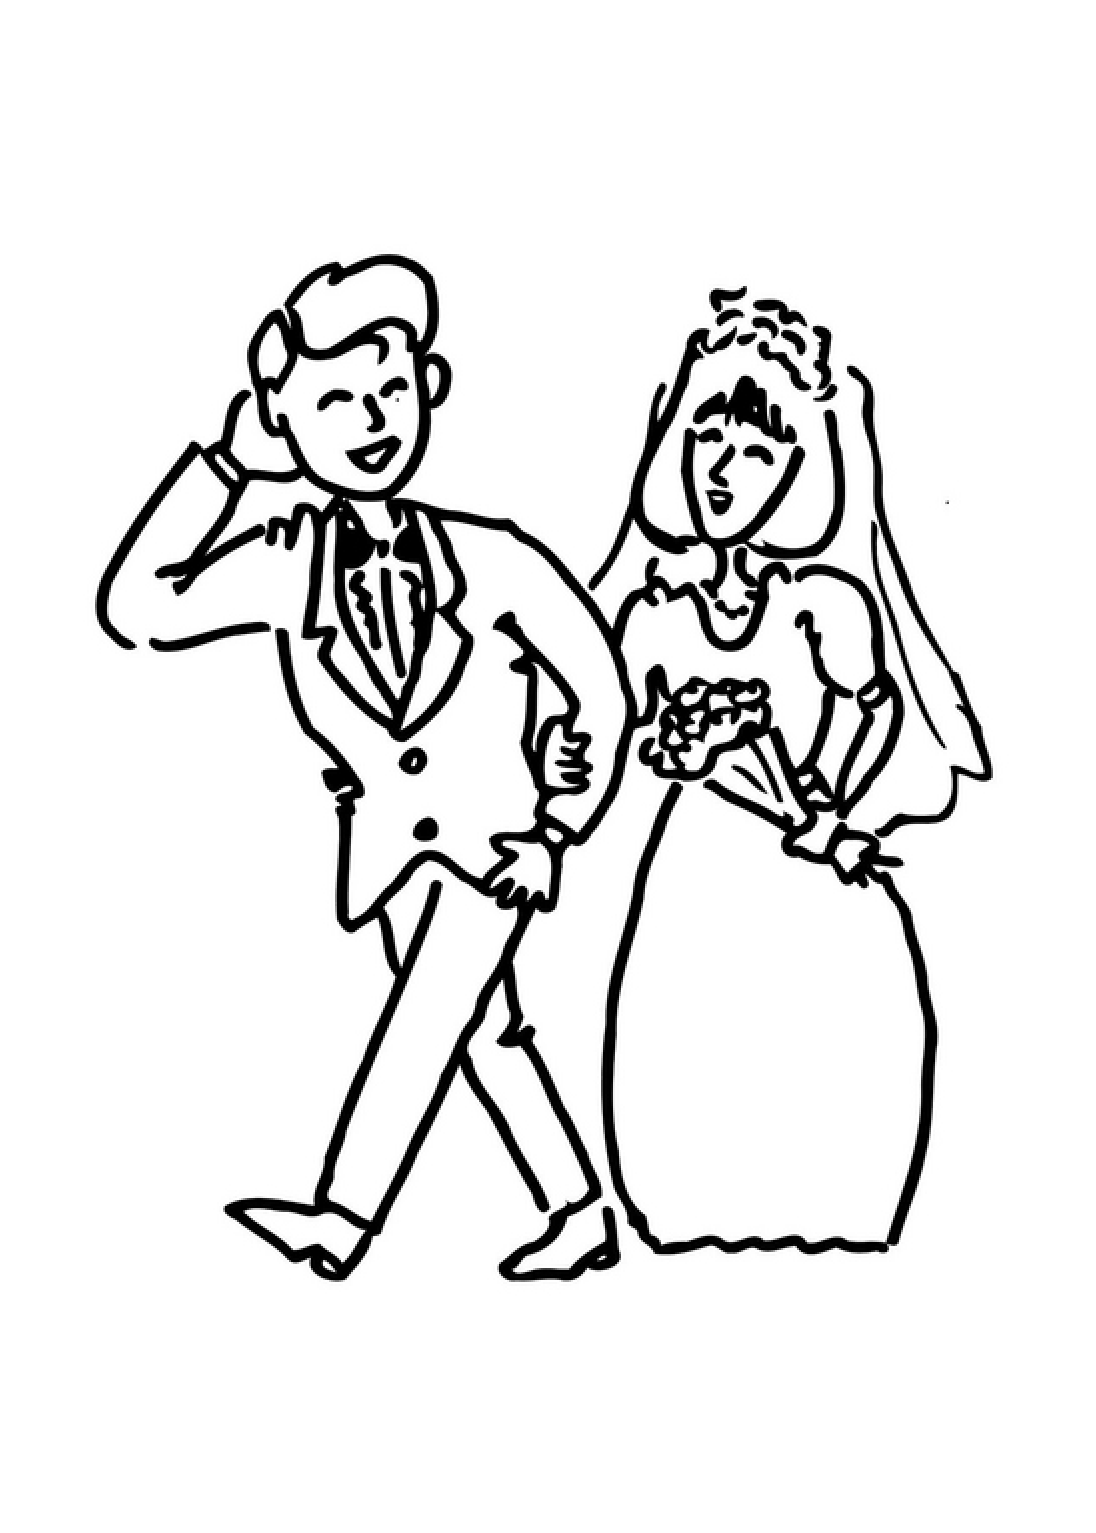
\includegraphics[scale=0.35]{../pernikahan-perkawinan/get-married.ps}\\
\camantra dan \camantri \\
Keluarga Bp. \keluargatra dan Bp. \keluargatri \\
oleh Romo \romo
} 
\date{18 April 2009}
\begin{document}

\maketitle
\Large  
\thispagestyle{empty}
%\newpage
%~~~ 
\newpage
\judul{RITUS PEMBUKA}

\lagu{Lagu pembukaan: \lagupembukaan}

\subjudul{Tanda Salib}
\BI{Dalam nama Bapa dan Putera dan Roh Kudus}
\BU{Amin}

\subjudul{Salam Pembukaan}
\BI{Rahmat Tuhan kita Yesus Kristus, cinta kasih Allah, dan persekutuan Roh Kudus beserta kita}
\BU{Sekarang dan selama-lamanya}

\subjudul{Pengantar}
\BI{Bapak, Ibu, dan Saudara-saudara, pada malam ini, malam menjelang pernikahan saudara \camantra dan \camantri ini, yang menurut adat Jawa, para bidadari turun dari kahyangan untuk memberi berkat, maka dinamakan \emph{midodareni}. Kita sebagai umat Katolik mengadopsi upacara ini dengan memohon agar Roh Kudus turun atas calon mempelai dan keluarganya. Kita memohon berkat dari Tuhan, 
agar calon mempelai dipenuhi oleh rahmat/karunia Allah agar dapat berfungsi sesuai dengan yang dikehendaki oleh Allah. }

\subjudul{Tobat}
\BI{Marilah kita hening sejenak untuk mempersiapkan diri dalam perayaan syukur ini sambil menyadari bahwa kita sering melupakan kebaikan Tuhan dan enggan mewartakan dan mewujudkan kebaikan tersebut melalui pikiran, perkataan, dan perbuatan kita.}

\BI{Saya mengaku}

\BU{Kepada Allah yang Maha Kuasa dan kepada saudara sekalian bahwa saya telah berdosa dengan pikiran dan perkataan, dengan perbuatan dan kelalaian. Saya berdosa, saya berdosa, saya sungguh berdosa. Oleh sebab itu saya mohon kepada Santa Perawan Maria, kepada Para Malaikat dan orang kudus dan kepada saudara sekalian, supaya mendoakan saya kepada Allah Tuhan kita.}

\BI{Semoga Allah Yang Maha Kuasa mengasihi kita, mengampuni dosa kita dan menghantar kita ke hidup yang kekal.}

\BU{Amin}

\lagu{Tuhan Kasihanilah Kami: \lagukyrie}

\subjudul{Doa Pembukaan}

\BI{Marilah kita berdoa,
Allah Maha Kasih, sumber ketentraman dan kebahagiaan orang berkeluarga, malam ini kami berkumpul atas nama Tuhan, memohon sudilah Engkau hadir, bersama para Malaekat dan para kudusMu di surga, menyaksikan dan memberi berkat pada pernikahan saudara \camantra dan \camantri, seperti saat Yesus bersama Ibu Maria dan para Rasul menghadiri dan memberkati perkawinan di Kana. Demi Kristus, Tuhan dan pengantara kami.}

\BU{Amin}

\judul{LITURGI SABDA}

\subjudul{Bacaan pertama: Kejadian 2:18-24}

\BP{\emph{Pembacaan dari Kitab Kejadian}

TUHAN Allah berfirman: "Tidak baik, kalau manusia itu seorang diri saja. Aku akan menjadikan penolong baginya, yang sepadan dengan dia."

Lalu TUHAN Allah membentuk dari tanah segala binatang hutan dan segala burung di udara. Dibawa-Nyalah semuanya kepada manusia itu untuk melihat, bagaimana ia menamainya; dan seperti nama yang diberikan manusia itu kepada tiap-tiap makhluk yang hidup, demikianlah nanti nama makhluk itu.
Manusia itu memberi nama kepada segala ternak, kepada burung-burung di udara dan kepada segala binatang hutan, tetapi baginya sendiri ia tidak menjumpai penolong yang sepadan dengan dia.

Lalu TUHAN Allah membuat manusia itu tidur nyenyak; ketika ia tidur, TUHAN Allah mengambil salah satu rusuk dari padanya, lalu menutup tempat itu dengan daging.
Dan dari rusuk yang diambil TUHAN Allah dari manusia itu, dibangun-Nyalah seorang perempuan, lalu dibawa-Nya kepada manusia itu.

Lalu berkatalah manusia itu: "Inilah dia, tulang dari tulangku dan daging dari dagingku. Ia akan dinamai perempuan, sebab ia diambil dari laki-laki."

Sebab itu seorang laki-laki akan meninggalkan ayahnya dan ibunya dan bersatu dengan isterinya, sehingga keduanya menjadi satu daging.

\emph{Demikianlah sabda Tuhan}
}

\BU{Syukur kepada Allah.}

\lagu{Lagu Pengantar Bacaan: \laguantarbacaan}

%\lagu{Bait Pengantar Injil}

\subjudul{Bacaan Injil: Markus 10: 1 - 9}

\BI{Tuhan sertamu}

\BU{Dan sertamu juga}

\BI{Inilah Injil Yesus Kristus menurut Santo Markus}

\BU{Dimuliakanlah Tuhan}

\BI{
Dari situ Yesus berangkat ke daerah Yudea dan ke daerah seberang sungai Yordan dan di situpun orang banyak datang mengerumuni Dia; dan seperti biasa Ia mengajar mereka pula.
Maka datanglah orang-orang Farisi, dan untuk mencobai Yesus mereka bertanya kepada-Nya: "Apakah seorang suami diperbolehkan menceraikan isterinya?"

Tetapi jawab-Nya kepada mereka: "Apa perintah Musa kepada kamu?"

Jawab mereka: "Musa memberi izin untuk menceraikannya dengan membuat surat cerai."

Lalu kata Yesus kepada mereka: "Justru karena ketegaran hatimulah maka Musa menuliskan perintah ini untuk kamu.
Sebab pada awal dunia, Allah menjadikan mereka laki-laki dan perempuan,
sebab itu laki-laki akan meninggalkan ayahnya dan ibunya dan bersatu dengan isterinya,
sehingga keduanya itu menjadi satu daging. Demikianlah mereka bukan lagi dua, melainkan satu.
Karena itu, apa yang telah dipersatukan Allah, tidak boleh diceraikan manusia."

Berbahagialah orang yang mendengarkan sabda Tuhan, dan tekun melaksanakannya.}

\BU{Sabda-Mu adalah jalan, kebenaran dan hidup kami.}

\subjudul{Homili}

\subjudul{Aku Percaya}

\subjudul{Doa Umat}

\BI{Tuhan Yesus Kristus, perkawinan dan hidup berkeluarga adalah panggilan atau kedudukan yang terhormat. Marilah kita mendoakan \camantra dan \camantri agar memperoleh kebahagiaan dalam hidup pernikahan dan hidup berkeluarga tumbuh dan menjadi sempurna di dalam Tuhan.}

\BP{Bapa di surga, Sungguh Kudus dan Mulia Engkau dalam persekutuan dengan Putera dan Roh Kudus. Dalam nama PuteraMu itu, kami berdoa dan memohon kepadaMu untuk mencurahkan Roh KudusMu itu, kepada saudara kami \camantra dan calon isterinya, \camantri. Semoga dengan ikatan sakramen pernikahan yang besok akan saling diterimakan mereka, mereka menjadi keluarga katolik yang baik dan meneladani keluarga Kudus dari Nazaret. Kami mohon:}

\BU{Kabulkanlah doa kami, ya Tuhan.}

\BP{Semoga pernikahan yang akan diselenggaran esok pagi
memberi kebahagiaan bagi orang tua dan kaum kerabat kami sehingga terjalin
ikatan persaudaraan yang erat dan saling membantu. Kami mohon:}

\BU{Kabulkanlah doa kami, ya Tuhan.}

\BP{Semoga kedua calon mempelai
senantiasa menghayati hidup pernikahan dalam cinta kasih dan damai, selalu
setia dan saling menolong sampai akhir hidup mereka sehingga rahmat dan
kebaikan Kristus bersinar dari rumah tangga mereka. Kami mohon:}

\BU{Kabulkanlah doa kami, ya Tuhan.}

\BP{Semoga cinta kasih mereka
diberkati oleh Tuhan dengan karunia yang berlimpah, sehingga anak-anak yang dianugerahkan
kepada mereka sungguh-sungguh menggembirakan hati kedua orangtuanya dan menjadi
pewaris gerejaMu di dunia ini. Kami mohon:}

\BU{Kabulkanlah doa kami, ya Tuhan.}

\BP{Bunda Maria, Ibu segala kaum beriman, Ratu Surgawi. Sampaikanlah doa ini ke hadirat PuteraMu yang tak akan menolakMu. Engkau tahu, ya Bunda, dinamika hidup berkeluarga yang berliku-liku dan penuh tantangan dan cobaan, oleh karena itu, Ibu, dampingilah setiap langkah mereka dengan doaMu, agar mereka selalu tabah, kuat dan setia kepada PuteraMu di setiap desahan nafas dan langkah kaki mereka di dalam mengarungi bahtera keluarga. Kami mohon:}

\BU{Kabulkanlah doa kami, ya Tuhan.}

\BP{Untuk keluarga, saudara dan teman-teman yang belum menemukan pasangan
hidup. Hiburlah mereka agar dalam masa penantian ini mereka justru menemukan
Dikau dan menyadari kehadiranMu. Berilah pasangan hidup yang baik kepada mereka
menurut kehendakMu. Kami mohon:}

\BU{Kabulkanlah doa kami, ya Tuhan.}

\BI{Demikianlah ya Bapa, doa-doa
yang kami panjatkan kepadaMu bagi kedua calon mempelai ini. Kami percaya Engkau akan
mendengarkan dan menerima doa-doa ini. Bimbinglah mereka dalam usaha
menciptakan keluarga Katolik yang berbahagia. Demi Kristus, Tuhan dan
Pengantara kami.}

\BU{Amin.}

\judul{LITURGI EKARISTI}

\subjudul{Persiapan Persembahan}

\lagu{Lagu persembahan: \lagupersembahan}

\subjudul{Doa Persembahan}

\BI{Allah Bapa kami di surga, terimalah persembahan yang kami hunjukkan untuk menyucikan perkawinan ini. Semoga mereka menikmati berkat-Mu dalam membangun keluarga. Demi Kristus pengantara kami}

\BU{Amin}

\subjudul{Prefasi}

\lagu{Kudus: \lagusanctus}

\subjudul{Doa Syukur Agung}

\subjudul{Bapa Kami}
\lagu{\lagubapakami}

\subjudul{Salam Damai}

%\lagu{Anak Domba Allah: \laguagnusdei }

\subjudul{Persiapan Komuni}

\lagu{Lagu Komuni: \lagukomuni}

\judul{RITUS PENUTUP}

\subjudul{Ucapan Terima Kasih}

\subjudul{Berkat}

\BI{Saudara sekalian, marilah kita mengakhiri misa syukur malam menjelang pernikahan saudara \camantra dan \camantri dari keluarga Bapak \keluargatra dan Bapak \keluargatri  dengan mohon berkat dari Tuhan.}
\BI{Tuhan sertamu}
\BU{Dan sertamu juga}
\BI{Semoga keluarga ini dan kita semua yang hadir di sini senantiasa dibimbing dan dilindungi dengan limpahan berkat dari Allah Yang Maha Baik. ($\dagger$) Atas Nama Bapa, Putra, dan Roh Kudus}
\BU{Amin}
\BI{Dengan demikian misa syukur malam menjelang pernikahan telah selesai.}
\BU{Syukur kepada Allah.}
\BI{Marilah pergi, kita diutus}
\BU{Amin}

\lagu{Lagu penutup: \lagupenutup}

%\subjudul{Renungan - Rintangan di perjalanan}
%
%Ada sekelompok orang yang sedang mengadakan perjalanan. Di tengah jalan mereka menemukan sebatang besi yang menghalangi jalan. Setelah berunding masing-masing diberi kesempatan untuk menyingkirkan besi penghalang itu.
%
%Yang pertama Palu. Ia langsung memukul, memukul-mukulkan kepalanya. Akhirnya kepala palu melesat lepas dari tangkainya.
%
%Yang kedua Gergaji, chin saw. Ia mulai meraung-raung, berisik, dan membuat keributan. Dipasanglah gigi-giri gergaji itu pada batang besi. Tetapi gigi-gigi gergaji seketika rontok semua.
%
%Yang ketiga Kapak. Sejenak kapak hening, untuk mengasah mata kampak. Lalu Kampak hendak menghancurkan batang besi itu, tetapi dirinya sendirilah yang rusak.
%
%Akhirnya yang keempat, Api. Dengan lembut api itu memeluk batang besi, memanasinya. Dan lelehlah batang besi itu. Tersingkirlah halangan di jalan. Dan   mereka bisa meneruskan perjalanan.
%
%Api itu adalah api Roh Kudus, api cintakasih yang membakar hati kita. Datanglah Roh Kudus, masuklah dalam hati kami, agar kami semua mengalami bahwa Allah adalah kasih. 
%
%Terpujilah Tuhan Yesus untuk selama-lamanya. Amin.

\newpage
\thispagestyle{empty}
\judul{Ucapan Terima Kasih}
\begin{center}
%
\includegraphics{images}

Dengan penuh rasa syukur kepada Allah, terima kasih yang tulus kami haturkan kepada:

Romo \romo \vspace{0.5cm}

Semua pihak yang telah membantu terselenggaranya \\
Perayaan Ekaristi Midodareni.\vspace{0.5cm}

Segenap kerabat dan handai taulan yang berkenan menghadiri\\
Perayaan Ekaristi Midodareni rumah ini.\vspace{0.5cm}

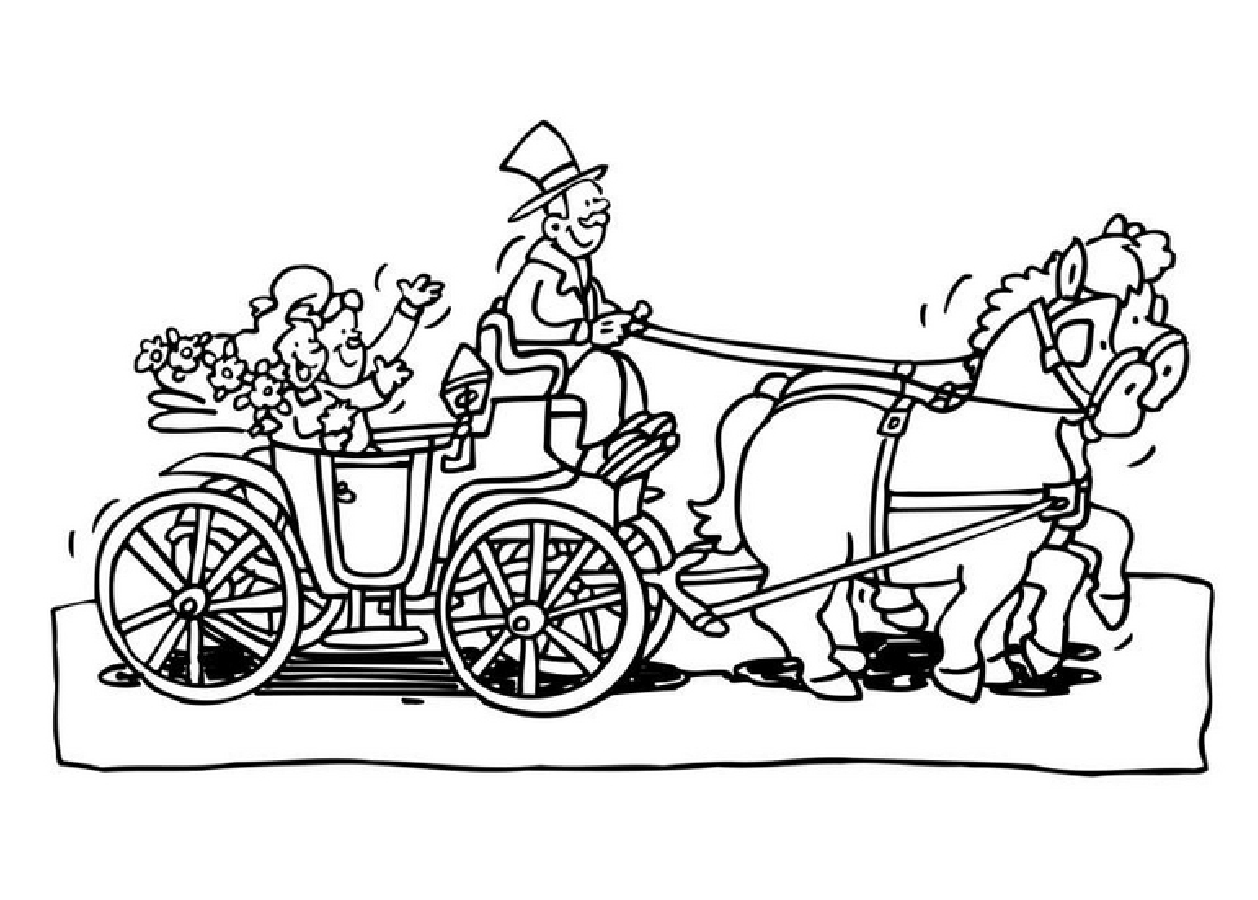
\includegraphics[scale=0.5]{../pernikahan-perkawinan/wedding-carriage.ps}
\end{center}



\end{document}
